\newpage
\subsection{ Описание обратной связи по току }
Согласно требованиям задачи, необходимо обеспечить скорости переброски системы не менее
$ \dot{q}_{max} = 1.73 $ рад/c при выбранном на этапе энергетического расчета передаточном
отношении редуктора $ i_\text{ред} = 225 $. Отсюда очевидно, что минимальное время импульса управления:

$$
    T_{y.min} = \frac{ 2 \cdot \pi }{ \dot{q}_{max} \cdot i_\text{ред} \cdot N_{r} \cdot p_{sm} \cdot 2 }
    = \frac{ 2 \cdot \pi }{ 1.73 \cdot 225 \cdot 50 \cdot 2 \cdot 2 }
    = 8.07 \cdot 10^{-05} ~c
$$

Это на 2 порядка отличается от электрической постоянной времени фазы $( \simeq2 \cdot 10^{-3} )$.
Для обеспечения максимально возможного момента на скоростях, близких к максимальной, необходимо
быстрое нарастание тока. Как было доказано ранее (\ref{ current_grow_estimate }), время роста можно
уменьшить, если увеличить напряжение.

\subsubsection{ Описание аппаратной части реализации токовой обратной связи }

\paragraph{ Схематика аппаратной части }

\begin{figure}[ht!]
    \centering
    \includegraphics[width=\textwidth, keepaspectratio, clip=true, trim=0mm 25mm 0mm 25mm]
                    {./src/pictures/current_measuring_sheme}
    \caption{Электрическая схема датчика тока}
    \label{pic_current_measuring_sheme}
\end{figure}

Датчик тока на плате управления выполнен на измерительном резисторе, последовательно
включенном в цепь каждой фазы. Так как управление происходит сигналом ШИМ, то имеем 4
датчика тока в кажом канале (A, B, C, D).
Сигнал с сериесного резистора, проходящий через RC-фильтр на измерительном резисторе и паралельно включенном
конденсаторе, поступает на усилитель постоянного тока с форсирующим звеном на входе, после чего поступает на АЦП.

Передаточная функция фильтра:
$$
    \frac{ U_\text{вых} }{ i_\text{н} } = \frac{ R_{53} }{ s R_{53} C_{59} + 1 }
$$

С полосой пропускания при наших параметрах $f_{RC.\text{проп} } \approx 15.915 ~\text{ГГц}$.

\newpage
\paragraph{ Аналого-цифровое преобразование }
В нашем распоряжении 12-разрядный аналого-цифровой преобразователь (далее АЦП) с 16-тью
мультиплексироваными вводами.
Имеет два канала измерения, которые могут использоваться как одновременно, так и последовательно.

\begin{itemize}
    \item \textit{Статическая погрешносaть}
        \begin{itemize}
            \item \textit{Аддитивная погрешность} \\
            Идеальная передаточная характеристика АЦП пересекает начало координат, а первый
            переход с нуля на единицу происходит при достижении значения 1 шаг. Аддитивная погрешность
            (погрешность смещения) может быть определена как смещение всей передаточной
            характеристики влево или вправо.
            \item \textit{Мультипликативная погрешность} \\
            Мультипликативная погрешность (погрешность полной шкалы) представляет собой разность
            между идеальной и реальной передаточными характеристиками в точке максимального
            выходного значения при условии нулевой аддитивной погрешности (смещение отсутствует).
            Это проявляется как изменение наклона передаточной функции.
            \item \textit{Дифференциальная нелинейность} \\
            У идеальной передаточной характеристики АЦП ширина каждой ``ступеньки'' должна быть
            одинакова. Разница в длине горизонтальных отрезков этой кусочно-линейной функции из
            $2^{n}$ ``ступеней'' представляет собой дифференциальную нелинейность.
            \item \textit{Интегральная нелинейность} \\
            Интегральная нелинейность (INL) - это погрешность, которая вызывается отклонением
            линейной функции передаточной характеристики АЦП от прямой линии.
            \item \textit{Погрешность квантования} \\
            Одна из наиболее существенных составляющих ошибки при измерениях с помощью АЦП -
            погрешность квантования - является результатом самого процесса преобразования.
            Погрешность квантования - это погрешность, вызванная значением шага квантования
            и определяемая как половина величины наименьшего значащего разряда.
            Она не может быть исключена в аналого-цифровых преобразованиях, так как является
            неотъемлемой частью процесса преобразования.
        \end{itemize}

    \item \textit{Случайная погрешность} \\
        Влияние этого рода погрешности на передаточную функцию идеального АЦП изображено на графике
        (рис. \ref{pic_adc_code_transition_noise})
        Случайные помехи содержат гармонические искажения, тепловой шум, шум квантования.
        Некоторые составляющие шума генерируются самим АЦП, некоторые могут поступать на вход АЦП
        из внешних цепей. Гармонические искажения, например, могут содержаться в измеряемом сигнале
        и одновременно генерироваться АЦП в процессе преобразования.

        \begin{figure}[!ht]
            \centering
            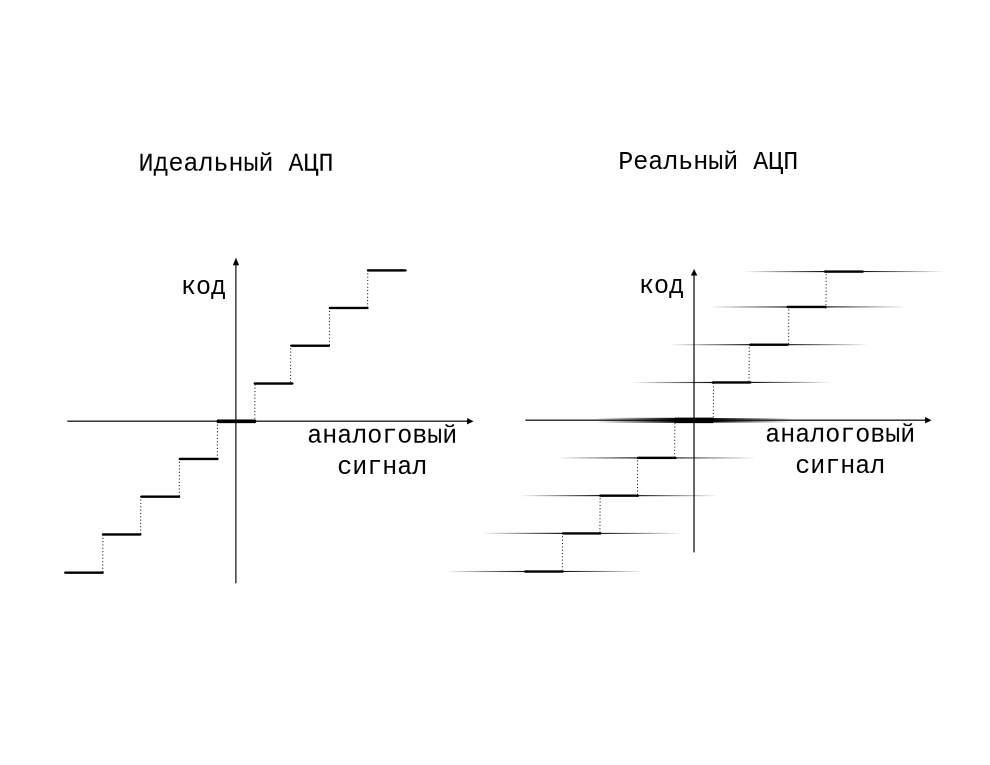
\includegraphics[width=0.7\textwidth, keepaspectratio, clip=true, trim=5mm 35mm 5mm 35mm]
                            {./src/pictures/adc_code_transition_noise}
            \caption{Случайная погрешность на выходе АЦП}
            \label{pic_adc_code_transition_noise}
        \end{figure}
\end{itemize}

\paragraph{ Методика оценки зашумленности сигналов с АЦП }
Самое значительное влияние по величине погрешности, как показывает практика, оказывают статические
погрешности в АЦП, но в используемом микроконтролере имеется схема внутренней калибровки, что позволяет
избавиться сразу от аддитивной и мультипликативной погрешности. Дифференциальная и интегральная
нелинейности имеют гораздо менее выраженый характер и не будет рассматриваться далее.

Оценить случайную погрешность измерений можно с помощью гистограммы множества измерений
входного сигнала, неизменного в течение эксперимента. В большинстве случаев получится
гистограмма нормального распределения или близкая к нему
(рис. \ref{pic_adc_noise_probabilistic_estimate}). Это позволит с некоторой точностью
оценить среднеквадратичное отклонение, а также, зная среднеквадратичное отклонение, количество
незашумленных разрядов как:

\begin{figure}[!ht]
    \centering
    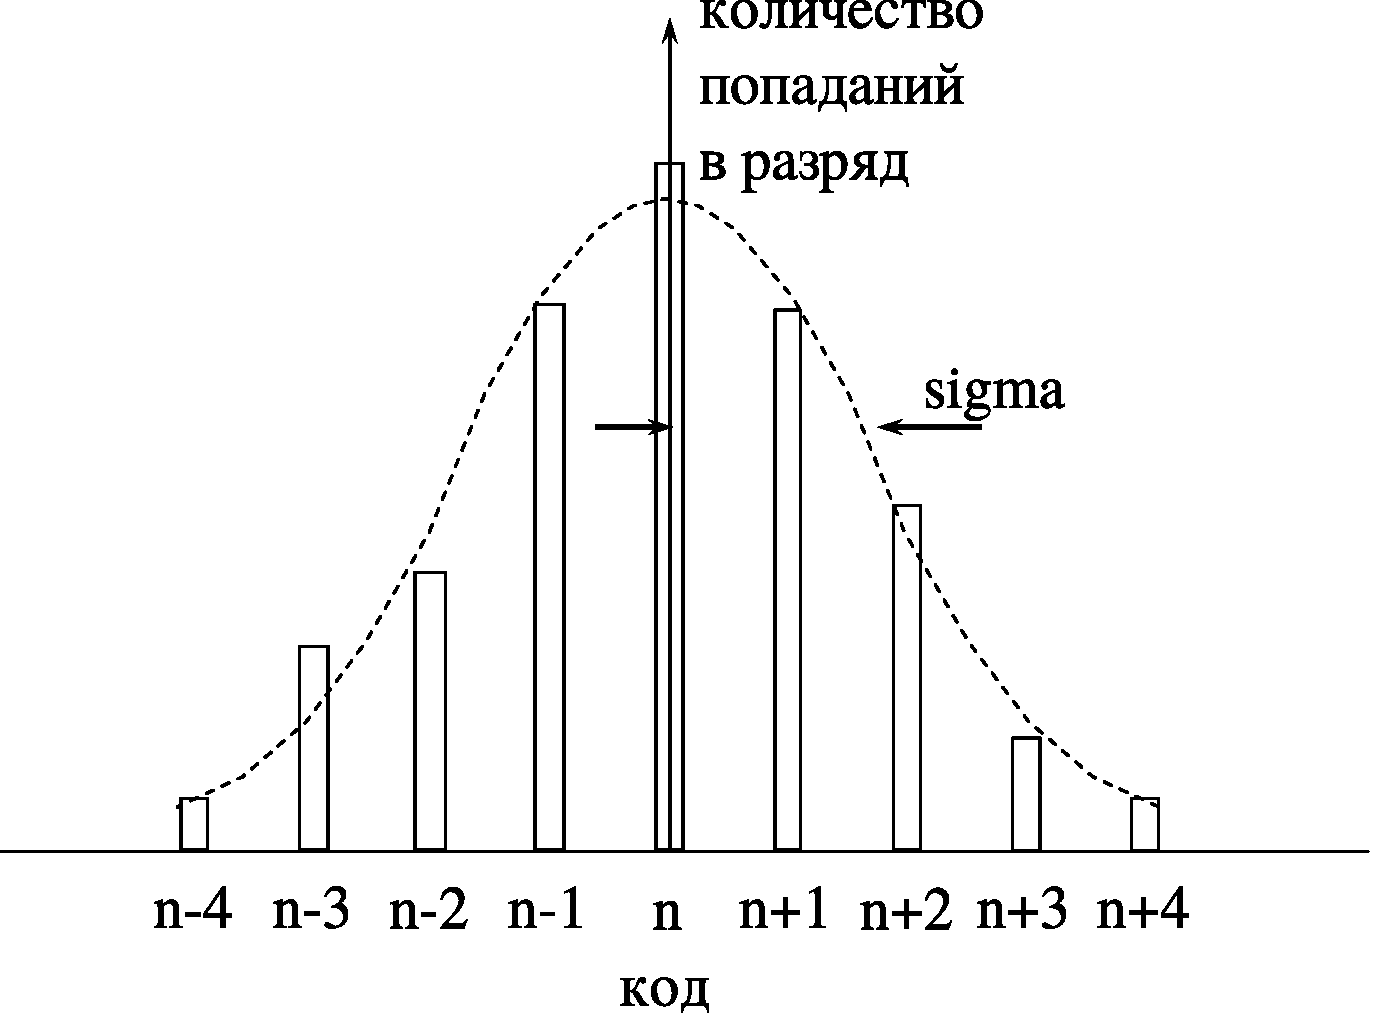
\includegraphics[width=0.5\textwidth, keepaspectratio, clip=true, trim=5mm 10mm 5mm 5mm]
                    {./src/pictures/adc_noise_probabilistic_estimate}
    \caption{Гистограмма распределения плотности вероятности шума АЦП}
    \label{pic_adc_noise_probabilistic_estimate}
\end{figure}

\begin{equation}
    \label{eq_noise_free_code_resolution}
    N_{noise free} = \log_{2}{( \frac{ 2^{N} }{ m_{adc} - p_{adc} } )}
\end{equation}

\begin{itemize}
    \item $ N $ - разрядность АЦП
    \item $ N_{noise free} $ - количество незашумленных разрядов
    \item $ m_{adc} $ - математичекое ожидание измеренного сигнала
    \item $ p_{adc} $ - максимальное значение измеренного сигнала
\end{itemize}

Самым примитивным и легко реализуемым фильтром будет простое отрезание шумящих разрядов,
но тогда значительно ухудшается разрешающая способность сенсора, что может
оказаться недопустимо в услових поставленной задачи. Для избежания подобоных проблем,
построим спектральную характеристику сигнала шума по уже полученным данным, по которой
построим цифровой фильтр.

\subsubsection{ Описание алгоритмической части реализации токовой обратной связи }

В рамках продолжения работы над данным проектом, в недалеком будущем планируется добавить
алгоритмическую фильтрацию сигналов в линии обратной связи по току. Данная фильтрация в
основном будет направлена на минимизацию шумов, классифицированных как несистемные.

\endinput
